% !TEX program = xelatex
\documentclass[utf8]{ctexbeamer}
\usetheme{Singapore}
\usepackage{amsmath}
\usepackage{hyperref}
\usepackage{graphicx}
% \usepackage{multicol} %用于实现在同一页中实现不同的分栏
\usepackage{ctex}

\begin{document}

\title{城市标度律的生成模型}
\author{修格致\ \ 1801110566 \\ \vspace{1cm} 导师\ \ 刘瑜 \ 教授}
\date{\today}



\begin{frame}
    \maketitle

\end{frame}

\begin{frame}{目录}
    \tableofcontents
\end{frame}

\section{绪言}

% \subsection{城市与规模}

\begin{frame}
    \begin{quote}
        城市的本质是规模经济。

        \flushright{-- Michael Batty}

        % 城市发展的不同阶段有着不同的性质,需要不同的建模方式。
        % \flushright{-- Gezhi Xiu}
    \end{quote}
\end{frame}

\begin{frame}{我国城市化的现状}

\begin{figure}
    \centering
    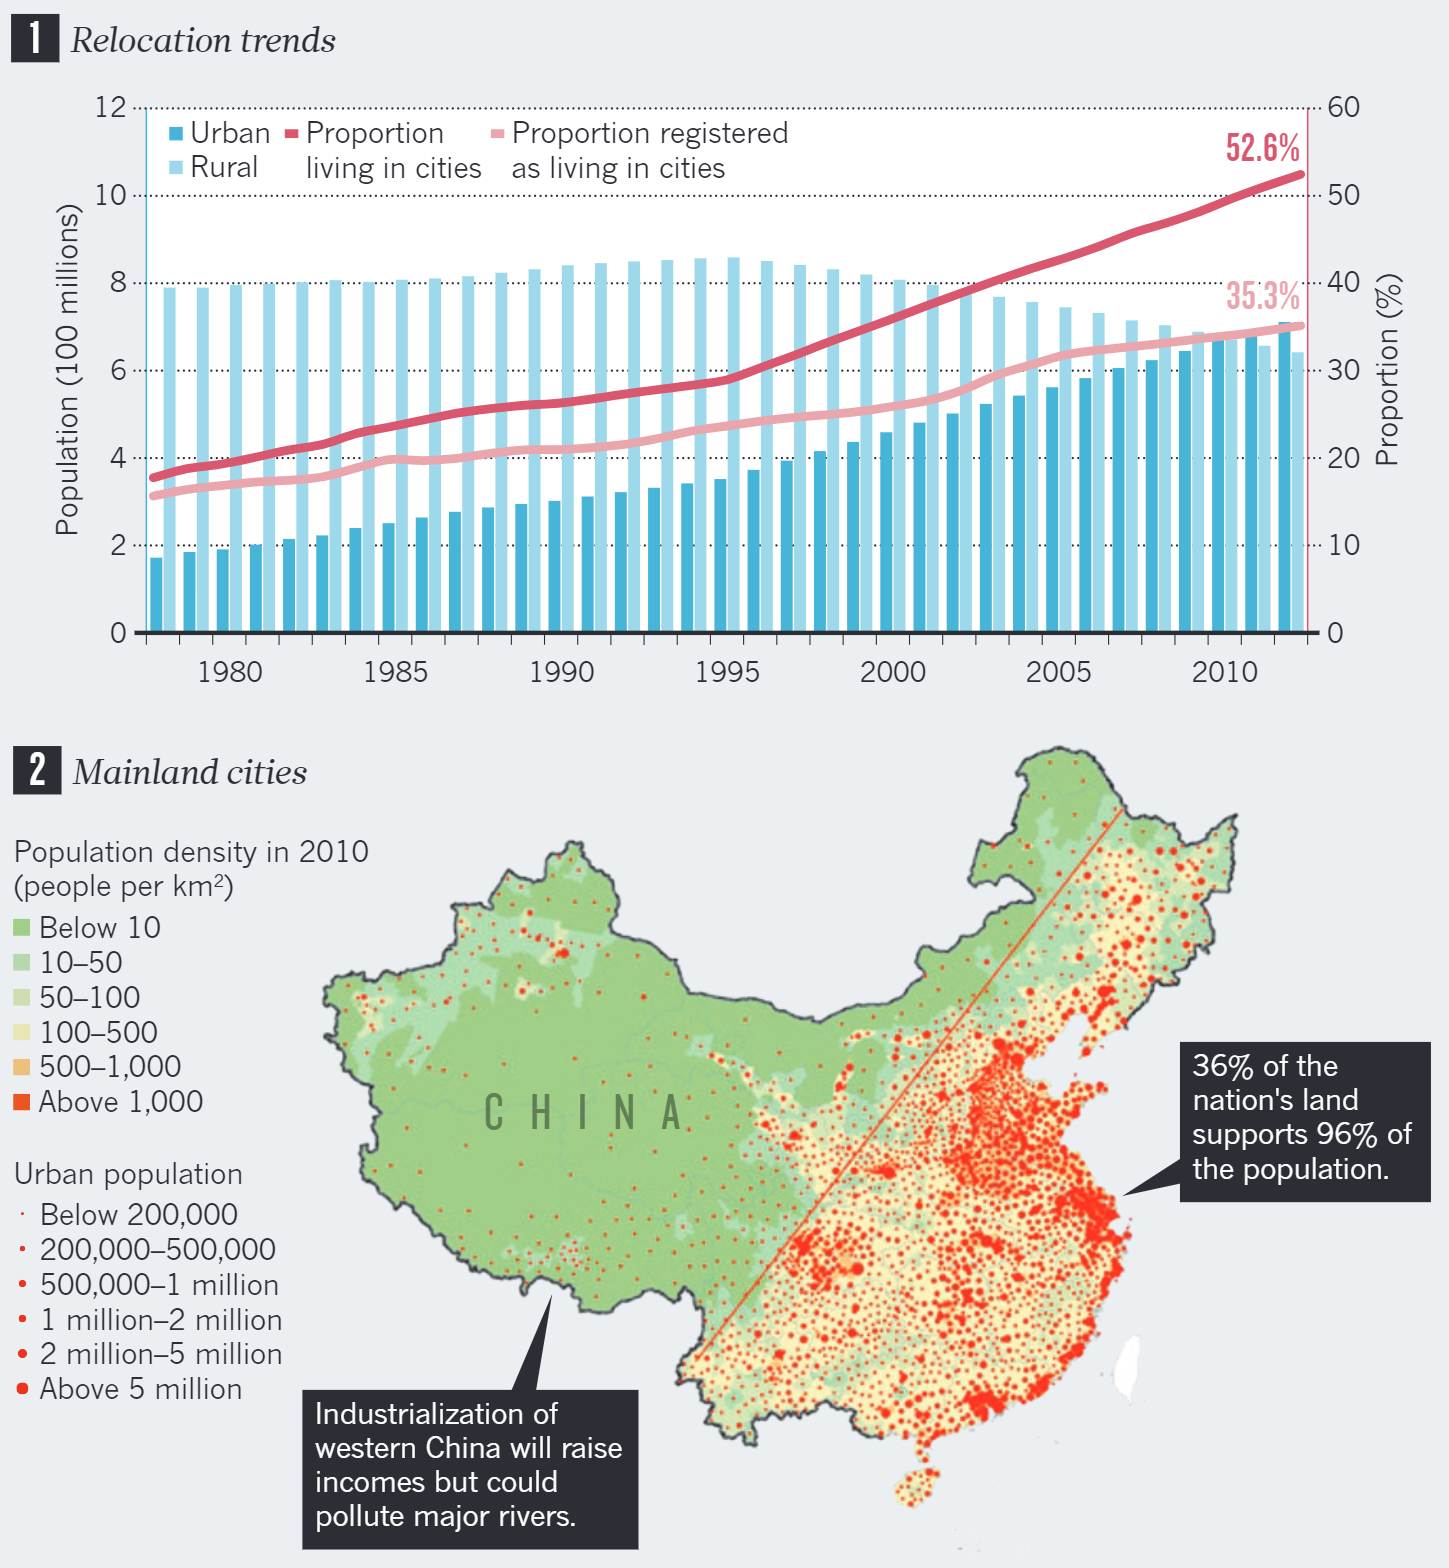
\includegraphics[width = 0.42\linewidth]{./图片/urban.png}
    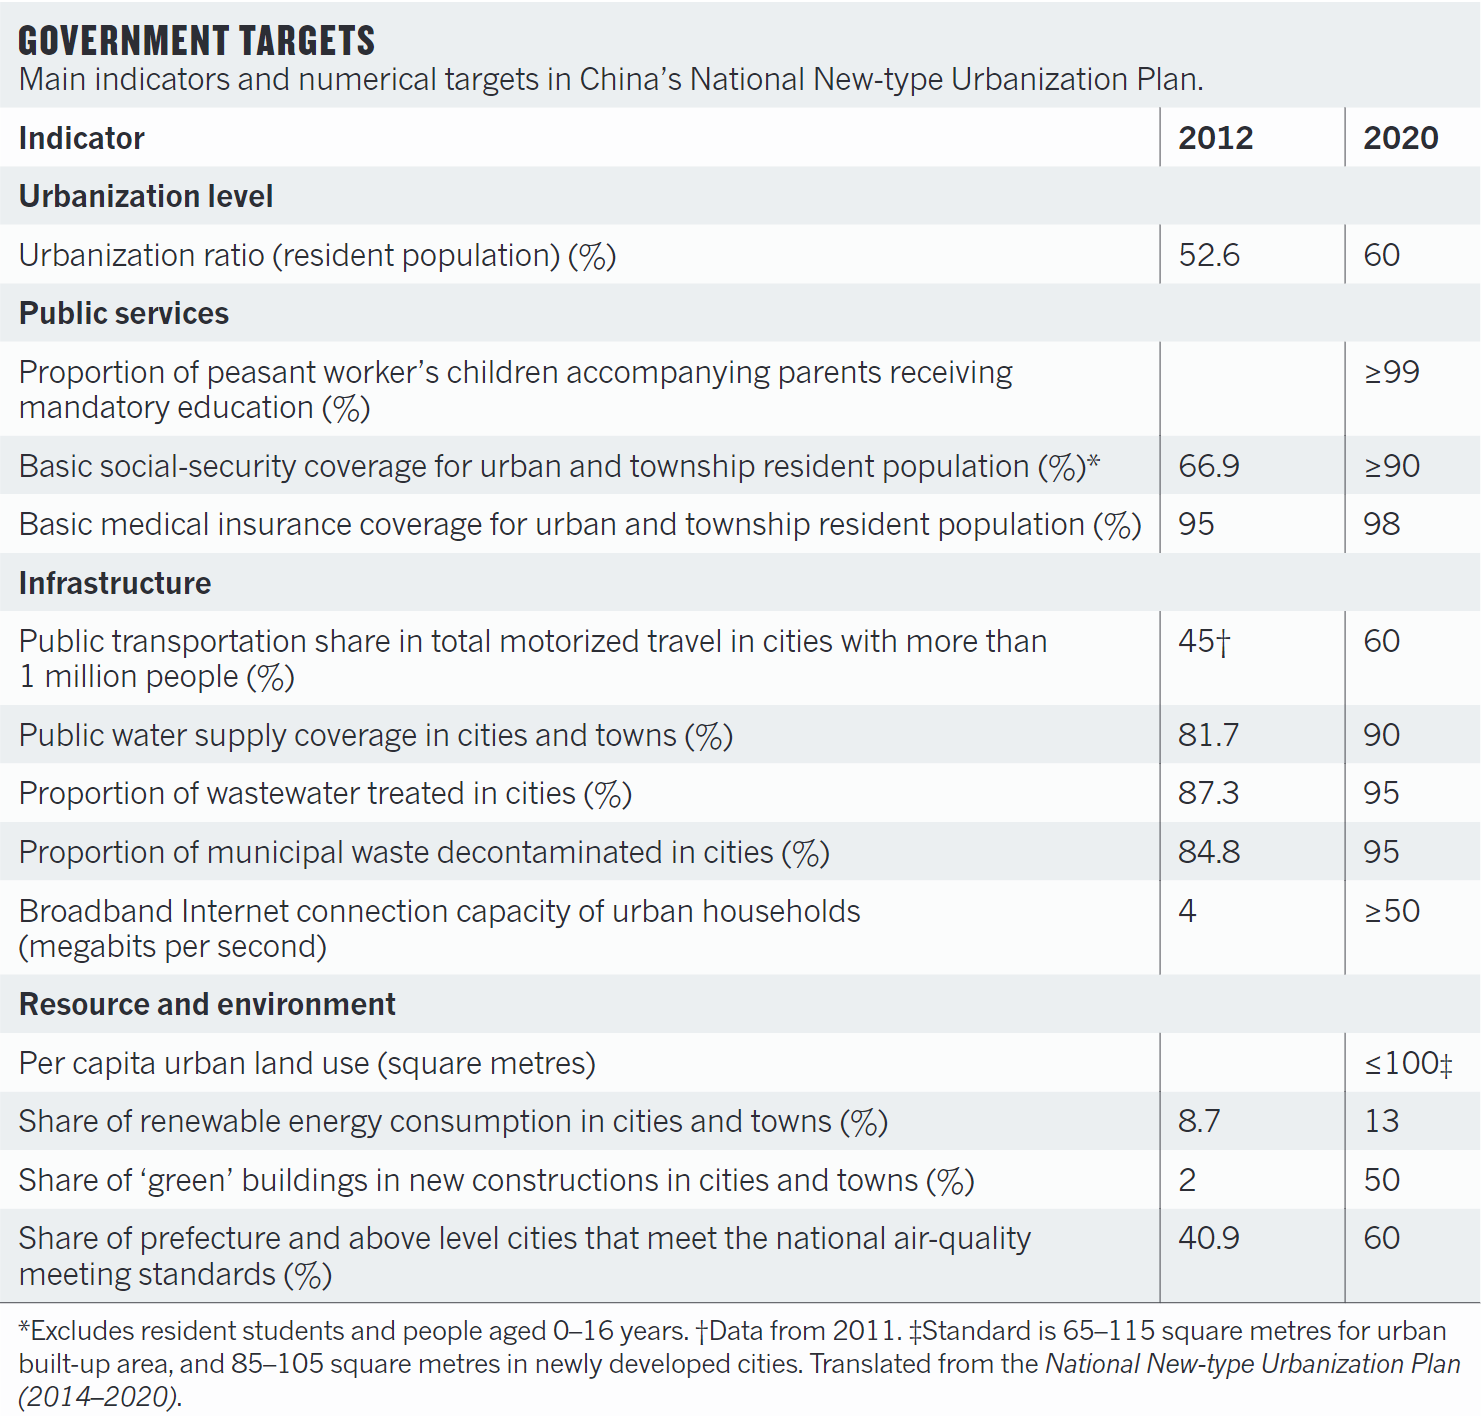
\includegraphics[width = 0.48\linewidth]{./图片/indicators.png}
    \caption{城市化的速度远快于人口增加的速度。Bai, X., Shi, P. \& Liu, Y. Society: Realizing China's urban dream. Nature 509, 158–160 (2014) doi:10.1038/509158a}
\end{figure}
\end{frame}

\begin{frame}{\textbf{现象}、原理、方法}
    \begin{itemize}
        \item 同一个区域内,往往人口越多,人均GDP越高
        \item 基础设施更新的速度慢于人口增长的速度
        \item 在全球的各个区域内,城市规模与位序的关系都类似
        \item 单中心的城市的城市内部人口分布服从指数衰减律
        \item ……
    \end{itemize}
\end{frame}

\begin{frame}{现象、\textbf{原理}、方法}
    \begin{itemize}
        \item 规模效应
        \item 政府行为响应社会需求
        \item 优势积累、富者愈富
        \item 人口扩散
        \item ……
    \end{itemize}
\end{frame}

\begin{frame}{现象、原理、\textbf{方法}}
    \begin{itemize}
        \item 主方程
        \item 率方程
        \item 马尔可夫生长
        \item 非马尔可夫限制生长
        \item ……
    \end{itemize}
\end{frame}

%\begin{frame}{城市科学}
    % 空间性
    % 经济属性
%\end{frame}

%%%%%%%%%%%%%%%%%%%%%%%%%%%%%%%%%%%%%%%%%%%%

\section{城市的涌现:聚集与变迁}

\begin{frame}{城市发展的历程}
    \begin{itemize}
        \item 城市涌现:吸引人口进入城市
        \item 城市完备化:城市空间拓展、产业进化
        \item 城市发展瓶颈:经济陷阱、空间限制……
    \end{itemize}
\end{frame}

\begin{frame}{城市化的动力}
    \begin{itemize}
        \item 城市比乡村生产效率更高
        \item 城市基础设施建设更加发达\footnote{Batty, M. (2013). The new science of cities. Mit Press.}
        \vspace{1cm}
        \item 城市对人更有吸引力
    \end{itemize}
\end{frame}

\begin{frame}{偏好依附}
    \begin{quote}
        \emph{流行性是有吸引力的。}\footnote{WWW and Internet models from 1955 till our days and the “popularity is attractive” principle, arXiv:cond-mat/0009090 [cond-mat.stat-mech]}。
    \end{quote}
\end{frame}

\begin{frame}{城市科学中的偏好依附}
    \begin{itemize}
        \item 人口迁移:
        \begin{itemize}
            \item 从农村到城市
            \item 城市间转移
        \end{itemize}
        \item 人口迁移到城市时,对城市的选择遵循\emph{偏好依附}原则:更倾向于迁移到人口更多/更发达的区域
        \begin{itemize}
            \item 新加入的人口会给城市更多发展资源,这会带来优势的积累,随后吸引更多的人到这个城市来,使这个城市的吸引力更强
            \item 结果:城市人口分布的标度律
        \end{itemize}
    \end{itemize}
    % \begin{figure}
    %     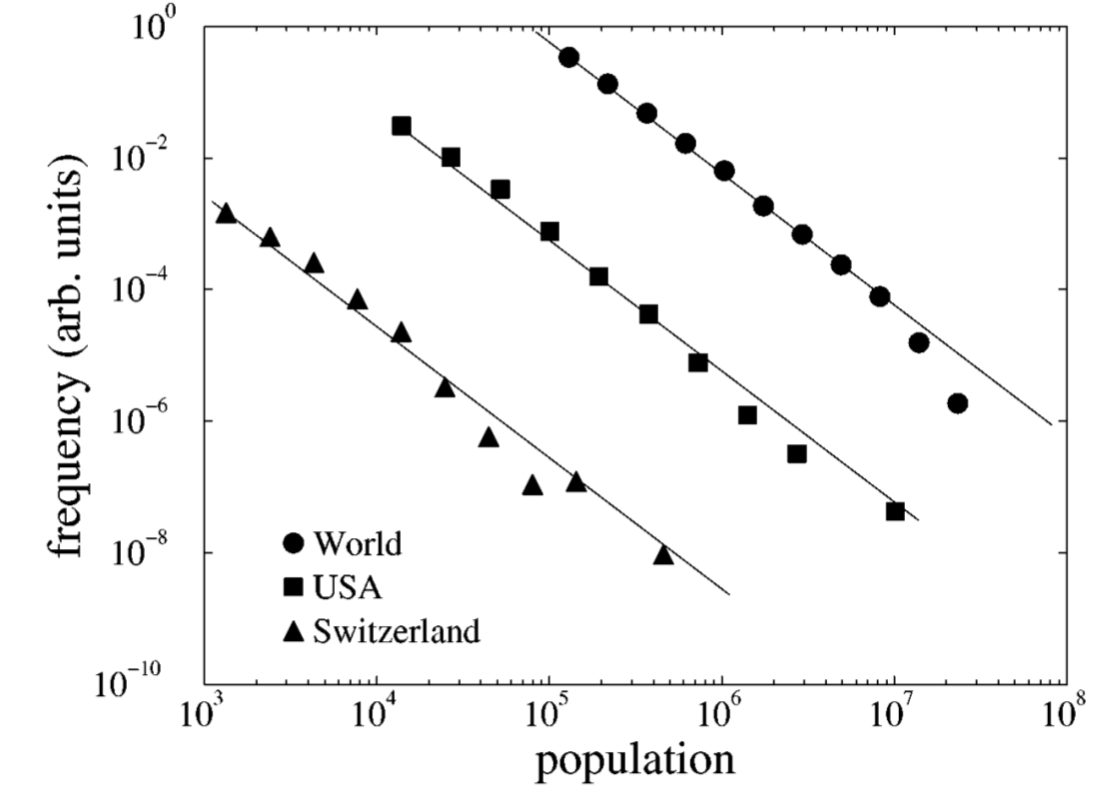
\includegraphics[width = 0.4\linewidth]{图片/roiiudreal.png}
    % \end{figure}
\end{frame}

\begin{frame}{城市科学中的偏好依附}
    刻画区域内城市形成机制的两类模型\footnote{左图:Modeling urban growth patterns, Nature volume 377, pages608–612(1995); 右图:Scaling behaviours in the growth of networked systems and their geometric origins, Scientific Reports volume 5, Article number: 9767 (2015)}:
    \begin{figure}
        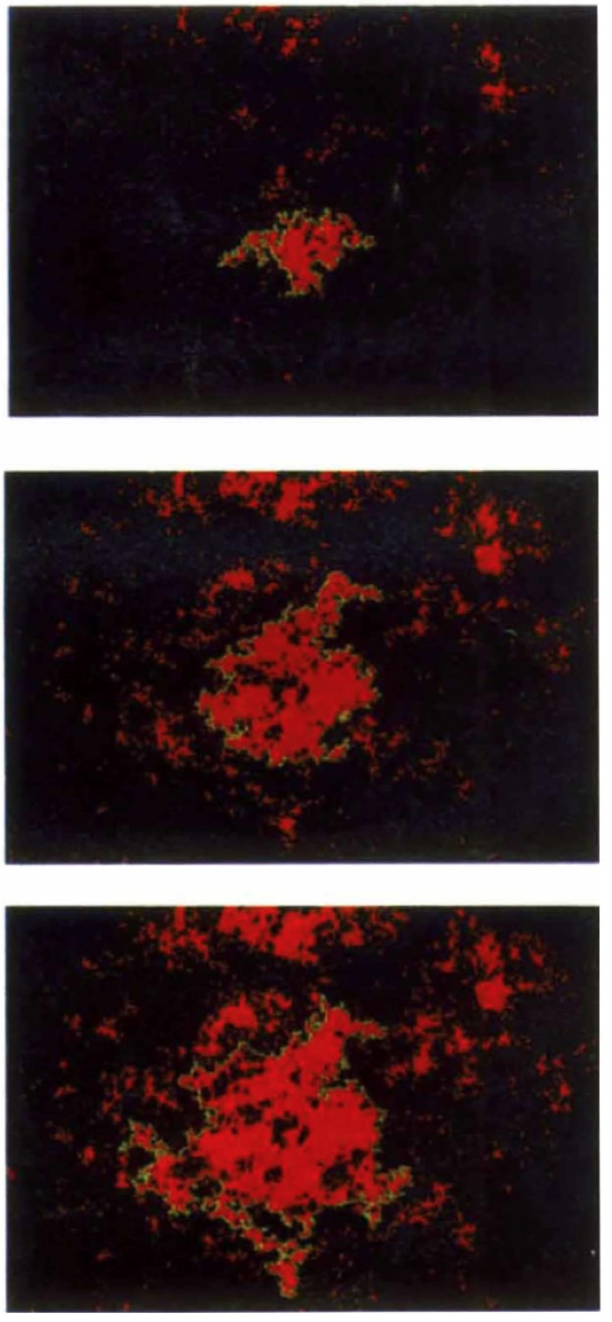
\includegraphics[width = 0.2\linewidth]{图片/mugp.png}
\hspace{1cm}
        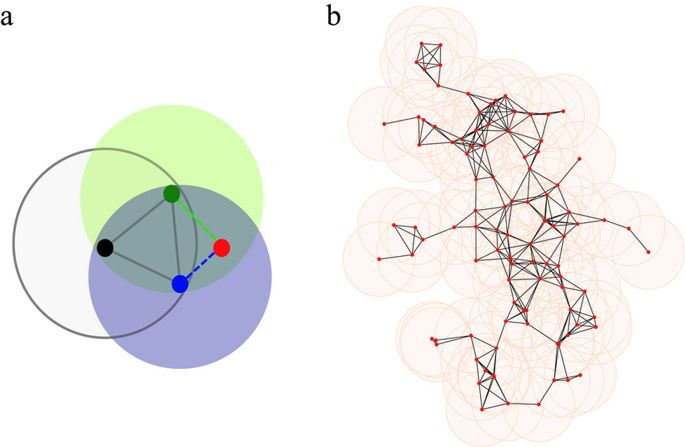
\includegraphics[width = 0.48\linewidth]{图片/srep09767-f1.jpg}
        \caption{考虑区域内总人口恒定:人口迁移; 
        只考虑城市人口:人口迁入}
    \end{figure}
\end{frame}

\begin{frame}{第一类:城市聚集体}
    \begin{itemize}
        \item 基础:晶格动力学模型
        \item 假定:
        \begin{itemize}
            \item 总人口恒定,初始分布均匀(同质化假设)
            \item 给定地块的基本分析单元
            \item 地理相关性通常被称为相关场,在模型中,作为局部人口迁移的动力存在
        \end{itemize}
    \end{itemize}
\end{frame}

\begin{frame}{第一类:城市聚集体}
    \begin{itemize}
        \item 过程
        \begin{enumerate}
        \item 记录每一个时刻$t$的每个格点$x$上的人口为$n(x,t)$. 则下一个时刻的人口分布符合\begin{align}
            n(x,t') = \begin{cases}
                (1-q)n(x,t)/p , \text{概率为 } p\notag\\
                qn(x,t)/(1-p) , \text{概率为 } 1-p
            \end{cases}
        \end{align}
        \item 每个格子上一定比例的人口扩散到八邻域上
    \end{enumerate}
        \item 这种机制保证了总人口的恒定,同时增加人口分布空间异质性。
        \item \textbf{解释}:农村迁入城市
    \end{itemize}
\end{frame}

\begin{frame}{第一类:城市聚集体}
    结果:标度律的出现
    \begin{figure}
        \centering
        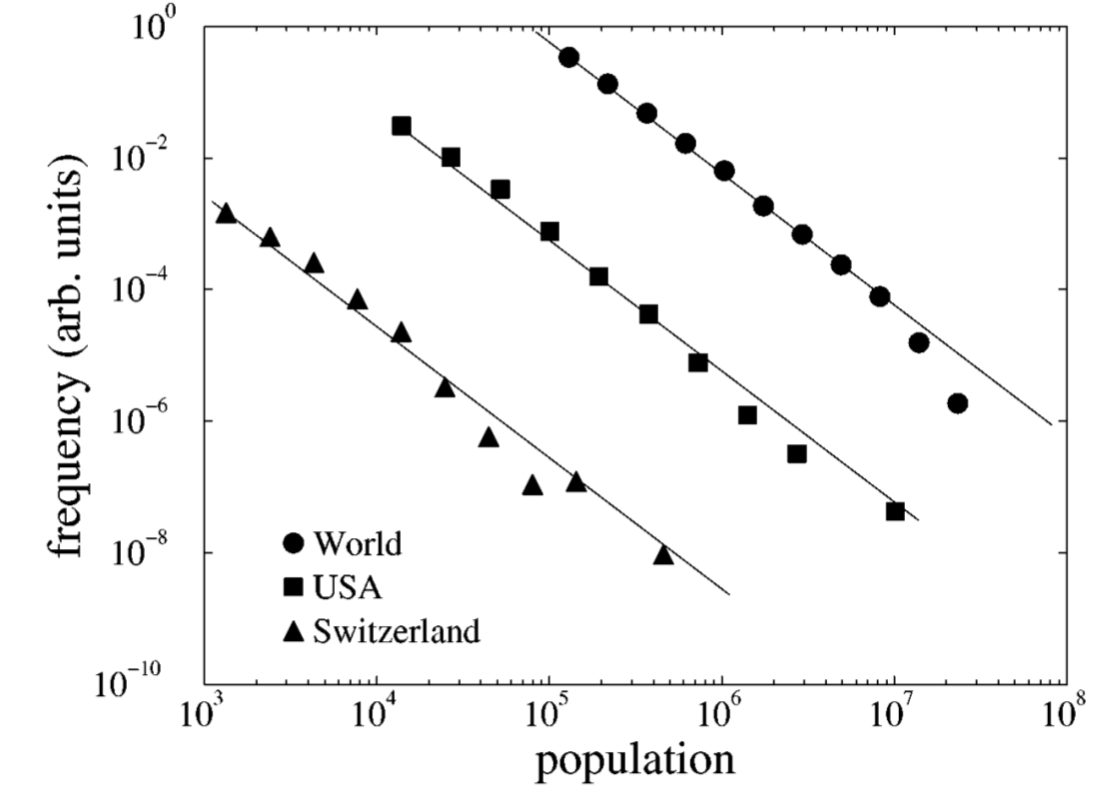
\includegraphics[width = 0.3\linewidth]{图片/roiiudreal.png}
        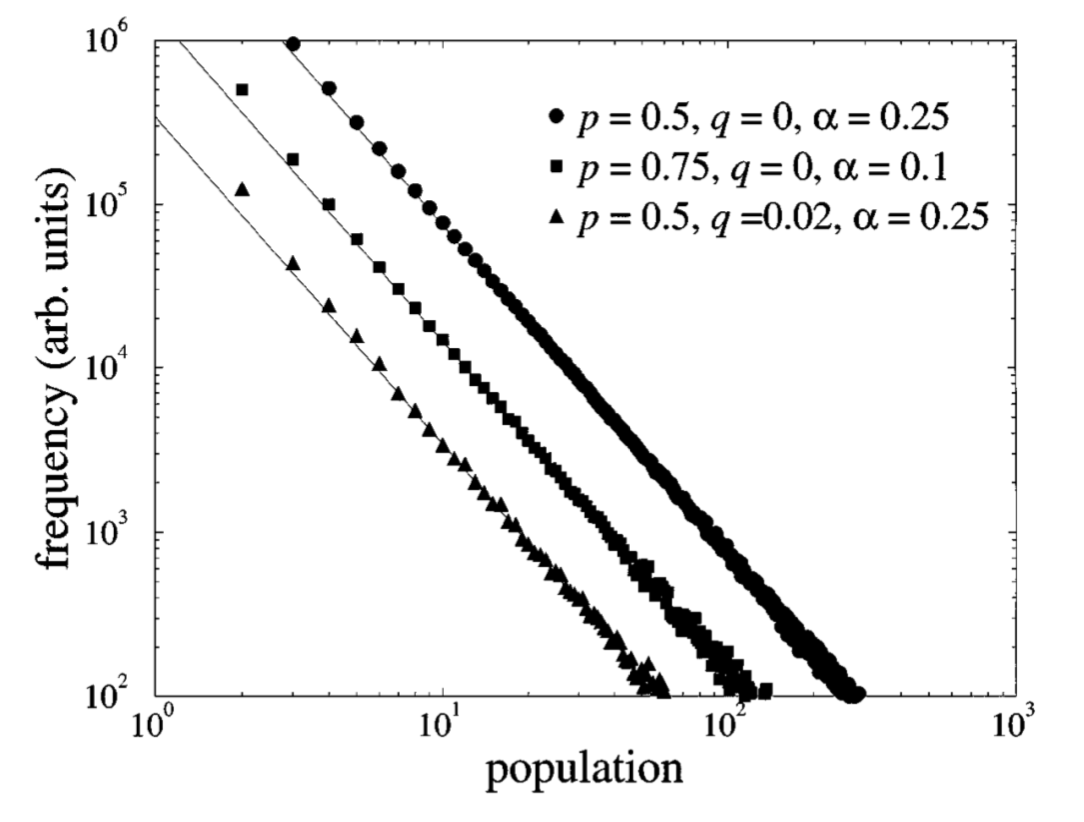
\includegraphics[width = 0.3\linewidth]{图片/roiiud.png}
        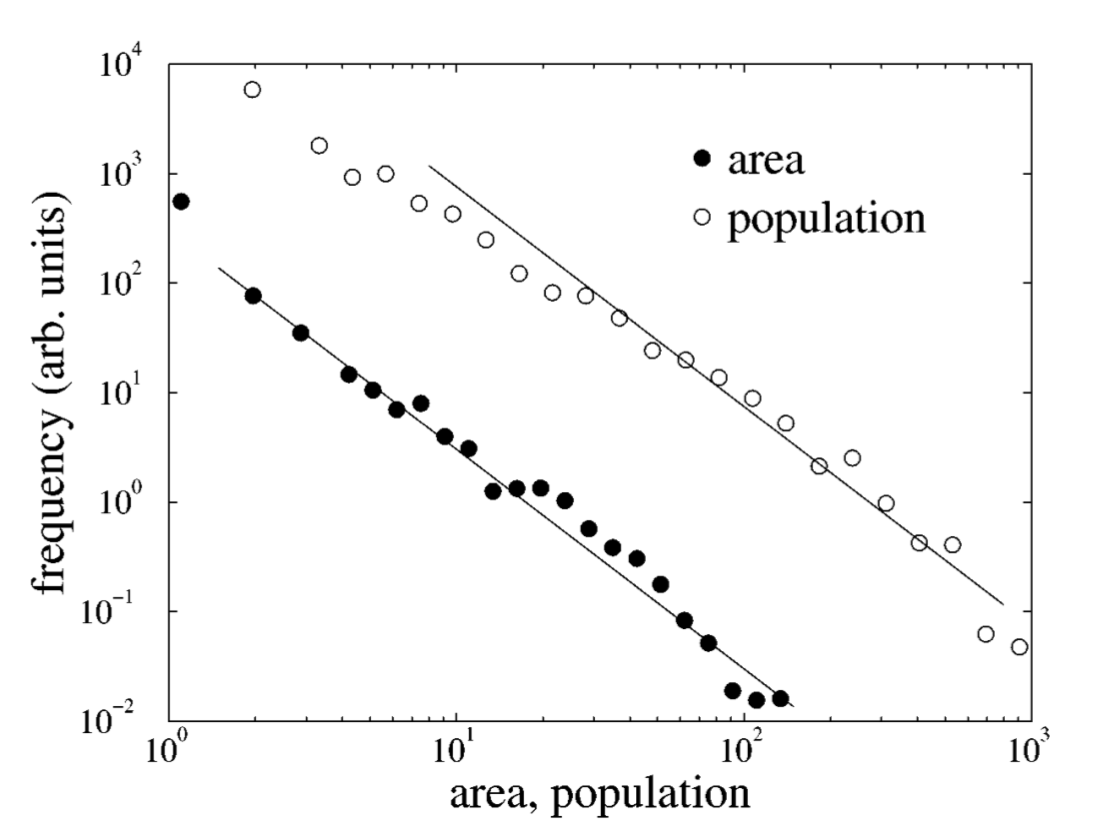
\includegraphics[width = 0.3\linewidth]{图片/roiiudarea.png}
        \caption{左图:全球2700个最大城市,美国的2400个最大城市和瑞士的1300个最大的自治市的人口分布\footnote{Role of Intermittency in Urban Development: A Model of Large-Scale City Formation
        Damián H. Zanette and Susanna C. Manrubia
        Phys. Rev. Lett. 79, 523 – Published 21 July 1997}. 图中斜率为$-2$ 右图是该文中对于不同的参数的三组模拟结果。我们发现,该模型下不同参数导出的城市人口的位序分布都服从一个参数为$2$的幂律分布。}
    \end{figure}
\end{frame}

\begin{frame}{第一类:城市聚集体}
    其他模型:Modelling urban growth patterns, Hernán A. Makse, Shlomo Havlin \& H. Eugene Stanley, Nature volume 377, pages608–612(1995)

    \begin{figure}
        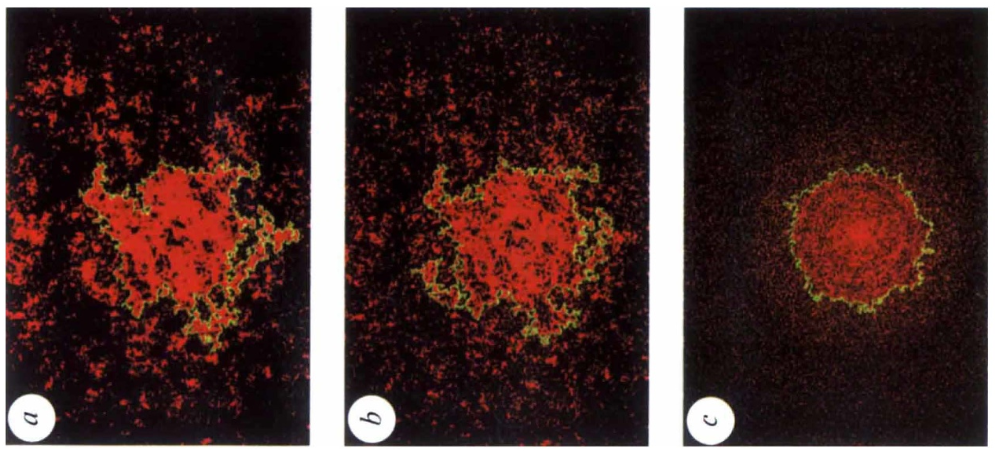
\includegraphics[width = 1\linewidth]{图片/modellingurbanpattern.png}
    \end{figure}
\end{frame}

\begin{frame}{第一类:城市聚集体}
    其他模型:Distance-weighted city growth, 
    Diego Rybski, Anselmo García Cantú Ros, and Jürgen P. Kropp
    Phys. Rev. E 87, 042114 – Published 16 April 2013

    \begin{figure}
        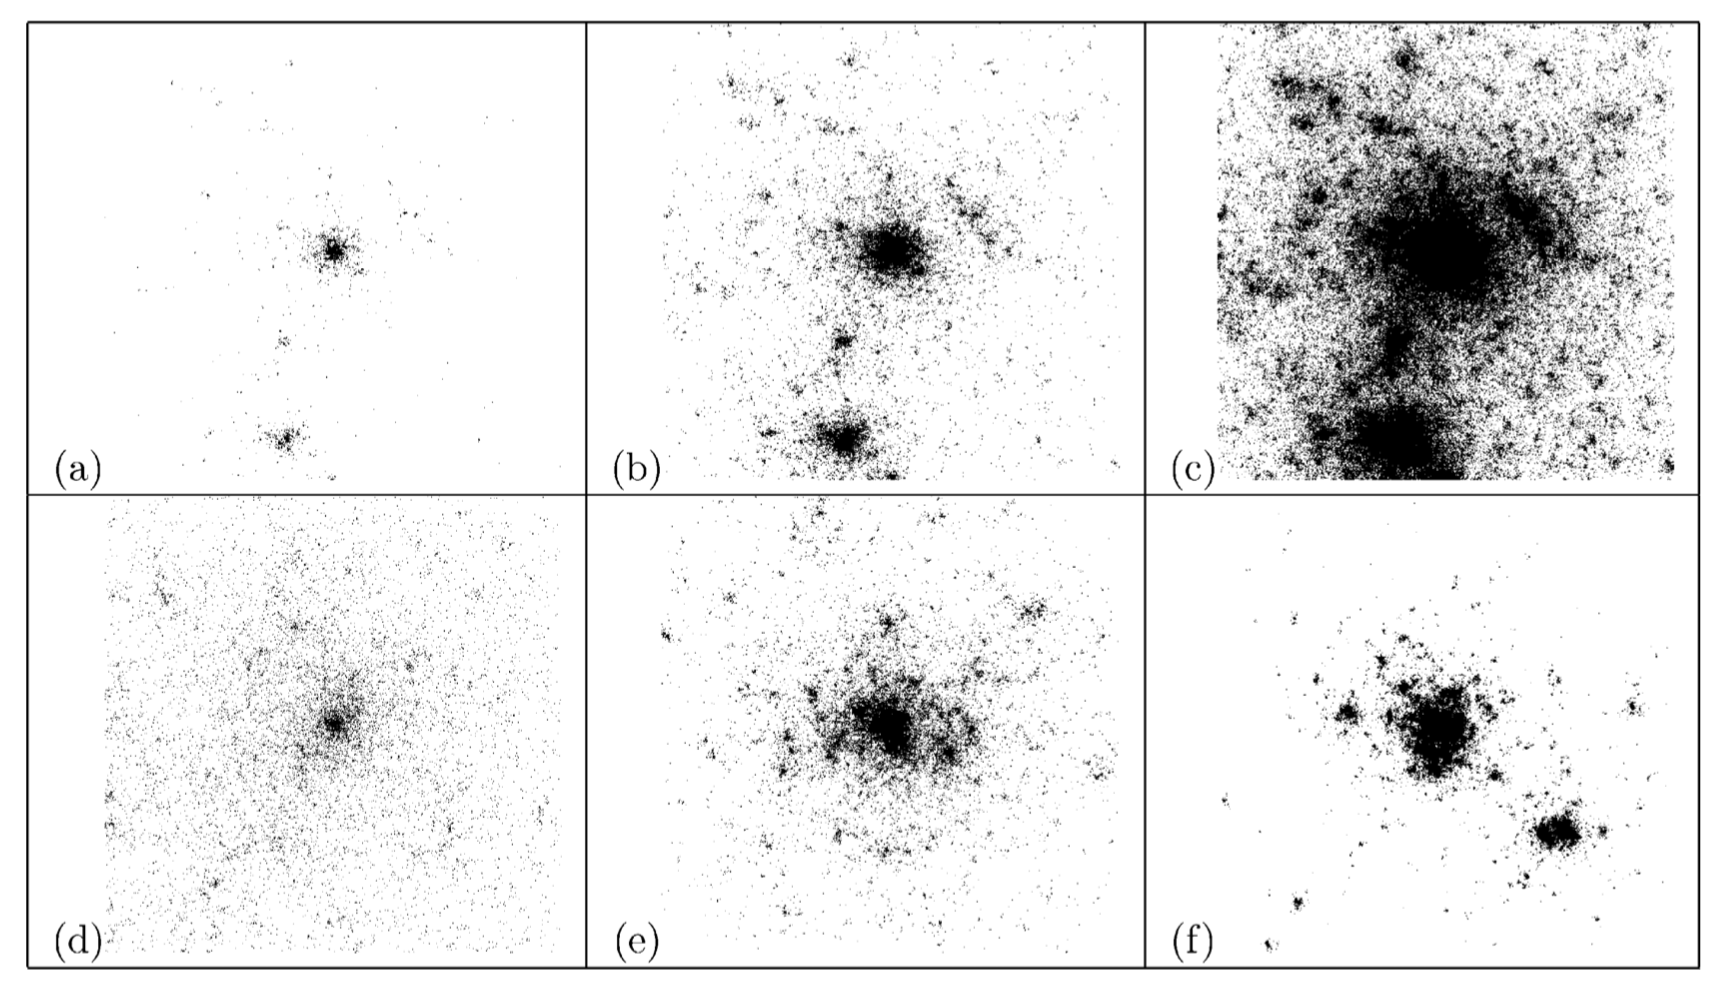
\includegraphics[width = 1\linewidth]{图片/distance-weighted.png}
    \end{figure}
\end{frame}

\begin{frame}{第一类:城市聚集体}
    其他模型:Laws of population growth, Hernán D. Rozenfeld, Diego Rybski, José S. Andrade Jr., Michael Batty, H. Eugene Stanley, and Hernán A. Makse

    \begin{figure}
        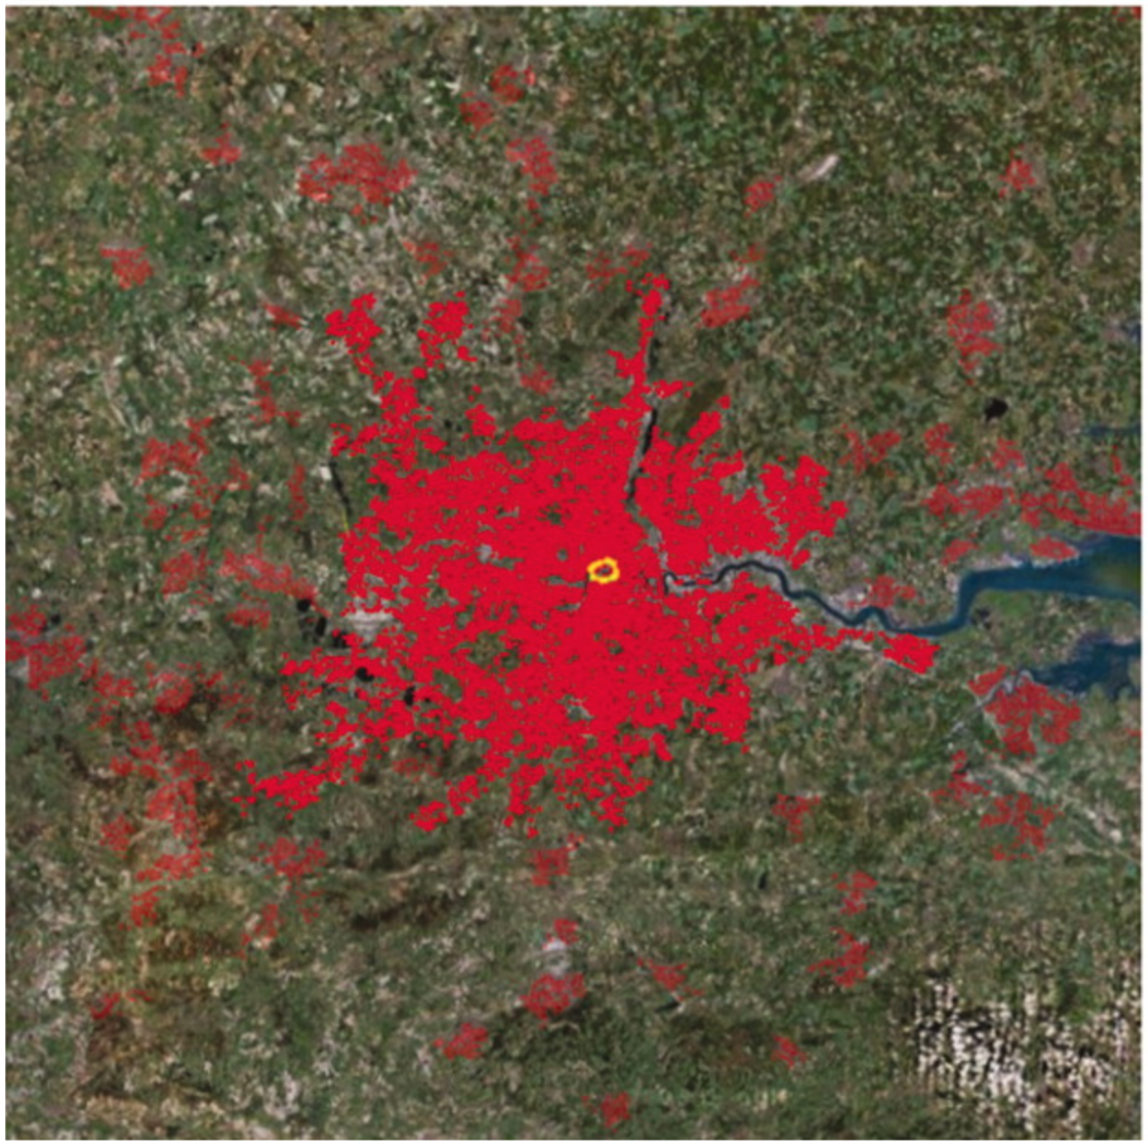
\includegraphics[width = 0.5\linewidth]{图片/cca.png}
    \end{figure}
\end{frame}

\begin{frame}{第一类模型:规律}
    \begin{itemize}
        \item 给定总人口的情况下,总物质是不变的。可以将城市的形成类比成星体的形成:\textbf{局部}聚集成城市。这般形成的城市体系往往具有标度律特征。
        \item 统计意义:城市聚合是一个\textbf{升矩}过程:总体人口密度不变,城市-乡村边界的人口密度分异增大。
        \begin{itemize}
            \item 由于乡村人口的自然扩散仍然是存在的,所以空间自相关程度不会达到完全负相关。
        \end{itemize}
    \end{itemize}
    \vspace{1cm}
    \textbf{空间异质性增强}:可以依照升矩/在城市直径尺度达到最大的“负空间自相关”,再添加其他必要的全局/城市内/乡村内性质,以构造新的生成模型。
\end{frame}

\begin{frame}{第一类模型:构造实例}
    比较目标格点与其八邻域人口均值($n_{neighbor}$)的相对大小更新格点人口数目,模拟人口迁入($\geq n_{neighbor}$)或迁出($n_{neighbor}$)过程。具体来讲,假设人口迁出比例为固定的$\alpha$,则目标区域的更新规则为:

\begin{equation}
n(x,t) 
\begin{cases}
	<\overline{n(\delta x,t)}: & n(x,t)=(1-\alpha)n(x,t) \notag\\
	 & n(\delta x,t) += \frac{\alpha}{8}n(x,t)\notag\\
	\geq\overline{n(\delta x,t)}: & no\ change
\end{cases}
\end{equation}
其中,$x$为目标格点,$\delta x$为其八邻域,$\overline{n(\delta x,t)}$为八邻域格点内的人口均值。人口数越多,区域的吸引力越强,就会有更多的人口迁入。在此模型中,更新只在目标格点人口低于邻域均值时进行。我们不考虑人口数值外的其它区域环境差异因素,因此低值格点会均匀地向其八邻域迁出$\frac{\alpha}{8}$比例的现有人口。
\end{frame}

\begin{frame}{第二类模型:空间生长模型}
    原理:
    \begin{itemize}
        \item 城市内部人口密度亦不是平均化的过程,有着特定的人口分布结构理论(Clark定律\footnote{Urban population densities
    C Clark - Journal of the Royal Statistical Society, 1951},同心圆理论\footnote{Roger E. Backhouse (2003) Concentric circles of limits to the rate of accumulation: an interpretation of Joan Robinson's theory of economic dynamics, Review of Political Economy, 15:4, 457-466}等)。
        \item 这些分布在区域范围内的意义:城市接纳外来人口的能力。
    \end{itemize}
\end{frame}

\begin{frame}{第二类模型:空间生长模型}
    匹配增长模型\footnote{Zhang, J., Li, X., Wang, X. et al. Scaling behaviours in the growth of networked systems and their geometric origins. Sci Rep 5, 9767 (2015)}。
    \begin{itemize}
        \item 定一个有界\(d\)维欧式空间\(S=|x_1|,\cdots,|x_d|\leq \frac{L}{2}.\) \(t=0\)时在原点插入一个结点
        \item 每个时刻\(t\),以均匀分布在\(S\)中放置一个新结点\(P_t\),记它的坐标为\(x_t.\) 如果存在一个已有结点\(P_q,q\in\{1,2,\cdots,t-1\}\),跟这个新生成的结点很接近,使得\(||x_p-x_q||< r\),则新结点\(P_t\)存活
        \item 连边机制为:将新加入结点与其\(r-\)临域的所有结点相连
    \end{itemize}
    \vspace{0.5cm}
    这个几何网络会加速增长。因为新加入的结点可生存的区域的测度(为所有存活结点的\(r-\)临域的开覆盖)会越来越大。
\end{frame}

\begin{frame}{第二类模型:空间生长模型}
    \begin{figure}
        \centering
        
        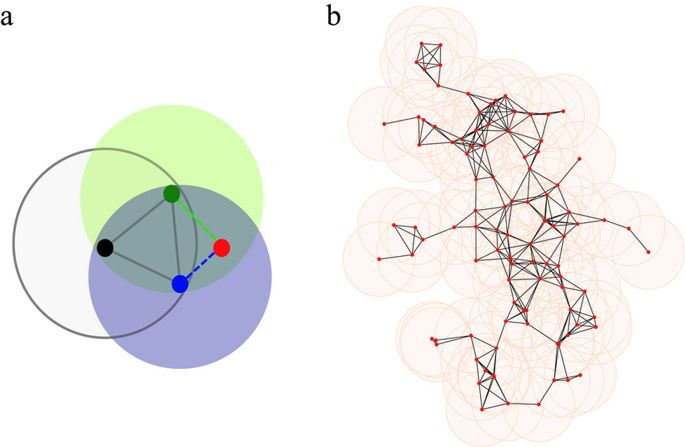
\includegraphics[width = 0.48\textwidth]{图片/srep09767-f1.jpg}
        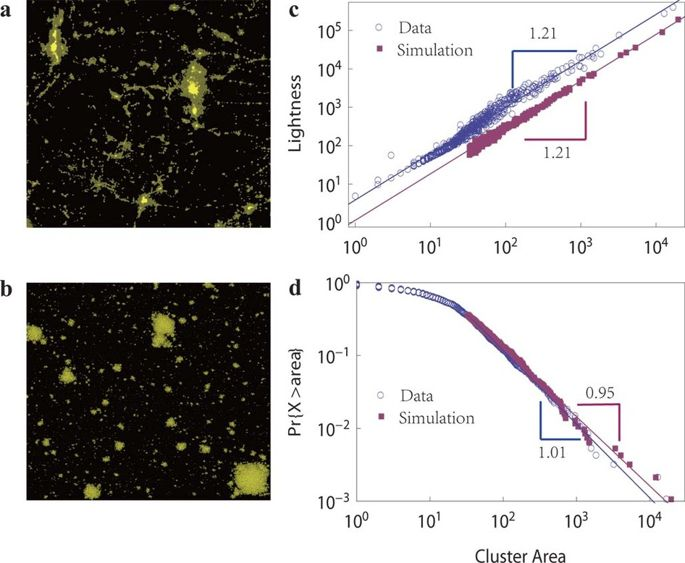
\includegraphics[width = 0.48\textwidth]{图片/srep09767-f3.jpg}
        \caption{左:匹配增长机制;右:a,b为模拟的图案、c为亮度密度、d为团块面积\footnote{Zhang, J., Li, X., Wang, X. et al. Scaling behaviours in the growth of networked systems and their geometric origins. Sci Rep 5, 9767 (2015)}}
    \end{figure}
\end{frame}

\begin{frame}{第二类模型:空间生长模型}
    Matching growth model\footnote{Zhang, J., Li, X., Wang, X. et al. Scaling behaviours in the growth of networked systems and their geometric origins. Sci Rep 5, 9767 (2015)}
    \begin{itemize}
        \item 城市半径\(R(t)\)(定义为\(\max\{||P_0-P_i||,i=1,2,\cdots t\}\))
        \item 到中心距离在\(\rho\)以内的结点个数\(\sim \rho^d\)
        \item 总人口:$N(t)\sim t^{d-1}$
        \item 边数:\(v(\rho,\Theta,t)\sim u(\rho,\Theta,t)^2\)(局部每两个边都相连),所以总边数可以写为$E(t) = t^{d+1}$.所以我们有$E(t)\sim N(t)^{\frac{d+2}{d+1}}$
        \vspace{0.5cm}
        \item 调整生存概率可以得到更适合真实世界的结果,使得结果更接近线性。
    \end{itemize}
\end{frame}

\begin{frame}{第二类模型:空间生长模型}
    基于人之间建立联系的方式\footnote{Gerald F. Frasco, Jie Sun, Hernán D. Rozenfeld, and Daniel ben-Avraham
    Phys. Rev. X 4, 011008 – Published 28 January 2014}的一个模型:假设有空间位置的人的之间的联系依赖于与这些“第二邻居”(即朋友的朋友)
    \begin{itemize}
        \item 给出一个社会联系的无标度网络
        \item Zipf律:高度联系的个体住在人口密度更高的区域,且取双对数图后所有点是落在同一条直线上
        \item 城市人口增长的Gibrat律(最近的真实数据验证了这个规律)
        \item 城市人口与人口密度的关系
        \item 社会联系与社会人口的超线性关系,即链接度高的人聚居的地方,人口亦多
    \end{itemize}
    一个可能的“变体”:依照(Kleinberg)小世界网络最优理论,即长距离的连接服从一个特定的幂律分布。(注意这个‘长距离’,这隐含着短距离的边可以不按幂律分布生成。)
\end{frame}

\begin{frame}{第二类模型:空间生长模型}
    Spatially Distributed Social Complex Networks\footnote{Gerald F. Frasco, Jie Sun, Hernán D. Rozenfeld, and Daniel ben-Avraham
    Phys. Rev. X 4, 011008 – Published 28 January 2014}
    \begin{figure}
        \centering
        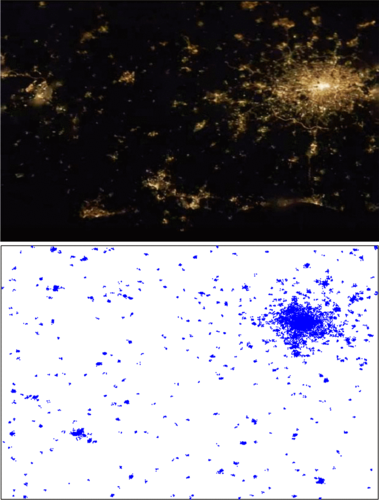
\includegraphics[width = 0.3\linewidth]{图片/medium.png}
        \caption{左图:英国南部城市夜光图像。右图:模型生成的城市图案。}
    \end{figure}
\end{frame}

% \begin{frame}{偏好依附机制的细节}
%     \begin{itemize}
        
%     \end{itemize}
% \end{frame}

\begin{frame}{偏好依附机制的细节}
    推导的两个工具:
    \begin{itemize}
        \item 率方程:单个主体的变化速率
        \item 主方程:比例变化关系
    \end{itemize}
    二者是分析系统组分数量关系的两个切入点
    \begin{itemize}
        \item 新加入资源更均匀分配给已有城市会使城市间贫富差距增大吗?
    \end{itemize}

\end{frame}

\begin{frame}{偏好依附机制的细节}
    最一般的:生长网络模型\footnote{Krapivsky, Redner, PhysRevE.63.066123}(Growing Network, GN)。该模型认为,刨除最初的几个结点,每次网络增加一个新结点的时候都会与已知的一个结点建立连边。选择已知结点的概率正比于已知结点的度(即连边个数)。
\begin{align} 
    \frac{dN_k}{dt} = \frac{A_{k-1}N_{k-1} - A_k N_k}{A} + \delta_{k,1},\notag
\end{align}其中$A_k=k$。由于每增加一个结点,总的度增加2,这个GN模型可以改写为\begin{align}n_k &= (k-1)n_{k-1}/2 - kn_{k}/2 \text{, for all }k \geq 2, \notag\\
    \Rightarrow n_k &= \frac{k-1}{k+2}n_{k-1}\notag\\ 
    \Rightarrow n_k &= \frac{6}{(k+2)(k+1)k}\cdot n_1\notag\\ 
    \Rightarrow n_k &\sim k^{-3}.
\end{align}
\end{frame}

\begin{frame}{偏好依附机制的细节}
    论文中的模型就到此为止了,但是我们发现,其中有一些值得注意的点可以探究。该模型的意义是新迁入的人口在某城市“扎根”,是由于他认识了某一个城市的原住民。我们可以进一步假设,他加入网络认识两个、三个、或者更多人的情形。通过相应地改写动力学方程,我们可以得到\begin{align}
        n_k = \frac{k-1}{k+2m}n_{k-1}\sim\frac{1}{C_{2m+k}^{k-1}}n_1\sim k^{-(2m+1)} \label{degm}
    \end{align}即如果一个人进入社会的时候,与更多人建立联系,则每个个体的度分布会更加偏态。这是一个很有启示意义的想法。即社会上的弱者不会因为新投入资源的增多而享受到更多公平。因为这种投入也降低了社会上强者不继续补强的概率。所以从人际资源的角度来说,新进入城市的人口随机地加入某一个特定人群,而不是多个社区,是最有利于社会公平的。
\end{frame}



%%%%%%%%%%%%%%%%%%%%%%%%%%%%%%%%%%%%%%%%%%%%
\section{城市的共性:产出与支持}

% \begin{frame}

%     \begin{quote}
%         人诗意地栖息在大地上。
%         \flushright{海德格尔}
%     \end{quote}
% \end{frame}

\begin{frame}{城市功能}
\begin{itemize}
    \item 城市集中建设基础设施,给市民提供了生活要素(衣食住行)。
    \item 市民在城市中以合作的方式工作,生产。创造一般等价物。
\end{itemize}
\end{frame}

\begin{frame}{立体社会:超线性与次线性}
    \(Y(N)\sim N^\beta \)
    \vspace{0.5cm}
    \begin{itemize}
        \item 城市优势的具体形式:一些城市指标(GDP、犯罪率等)关于人口超线性增长,即\(\beta>1\)
        \item 基础设施的建设关于人口是次线性的\footnote{Bettencourt, L., West, G. A unified theory of urban living. Nature 467, 912–913 (2010)},即\(\beta>1\)
        \vspace{0.5cm}
        \item 以人口数为自变量,不同的指标增长速度是不同的。
    \end{itemize}
\end{frame}

\begin{frame}{立体社会:超线性与次线性}
    \begin{figure}
        \centering
        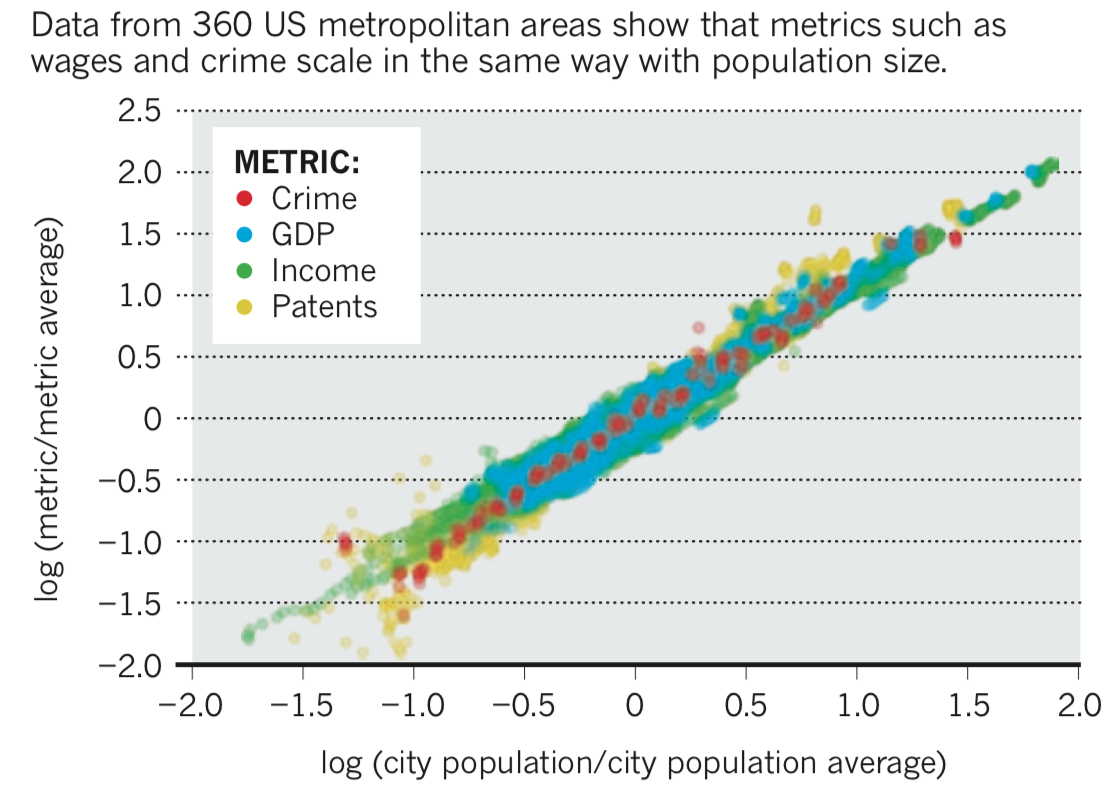
\includegraphics[width = 0.8\linewidth]{图片/scaling.png}
        \caption{Bettencourt, L., West, G. A unified theory of urban living. Nature}
    \end{figure}
\end{frame}

\begin{frame}{立体社会:超线性与次线性}
    \begin{itemize}
        \item 为什么城市指标很少是线性的?
        \begin{itemize}
            \item 一个可能的原因:这些指标建立的目的是衡量规模效应。
        \end{itemize}
        \vspace{0.5cm}
        \item 超线性与次线性是否都能理解为规模效应?
    \end{itemize}
\end{frame}

\begin{frame}{立体社会:超线性与次线性}
    \begin{itemize}
        \item 人的交互与合作带来超线性\footnote{Bettencourt, L., West, G. A unified theory of urban living. Nature};\textbf{对人来说,“产出”是超线性的}
        \item 基础设施的“交互与合作”带来设施对人口的超线性。以人为自变量时:基础设施是亚线性的。\textbf{对人来说,“需要”是亚线性的}
        \vspace{0.5cm}
        \item 城市是一个有层级的。城市是一个逐层供给的结构。
        \item 这是城市的不平凡之处。
    \end{itemize}
\end{frame}

\begin{frame}{寻找城市内部的不平凡之处}
    
    \begin{itemize}
        \item 超线性问题主要在城市内部:
        \begin{itemize}
            \item 城市是密集的空间实体。城市的组分交互频率比农村更高(大城市比小城市更高),会导致\textbf{产出}更多。
            \item 超线性问题的研究方法:生成模型
        \end{itemize}
        \item 亚线性问题更为广泛:机场(全国尺度)、加油站(城市内、城际尺度)、商场(城市内)
        \begin{itemize}
            \item 最优配置问题的解\footnote{Optimal design of spatial distribution networks, Michael T. Gastner and M. E. J. Newman
            Phys. Rev. E 74, 016117}
        \end{itemize}
    \end{itemize}
\end{frame}

\begin{frame}{工厂分布:亚线性的一个实例}
    \begin{figure}
        \centering
        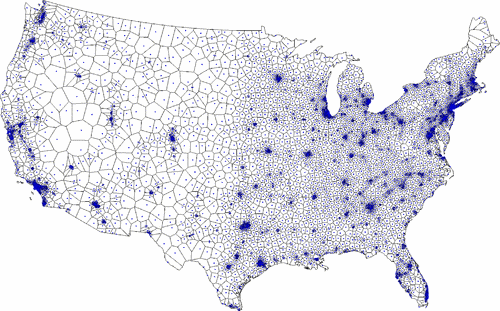
\includegraphics[width = 0.5\linewidth]{图片/distributednetwotk.png}
        \caption{美国某公司工厂在全国的分布}
    \end{figure}
\end{frame}

\begin{frame}{城市多中心性:场所“供给”市民的一个实例}
    交通拥堵可能是城市去中心化的一个原因。
    \flushright{-- Rémi Louf}
    \flushleft
    城市中心给市民提供了工作机会,所以城市中心供养了市民。这导致了市民数量对于城市中心的超线性性,即人口数对城市中心数的亚线性性。
    \begin{figure}
        \centering
        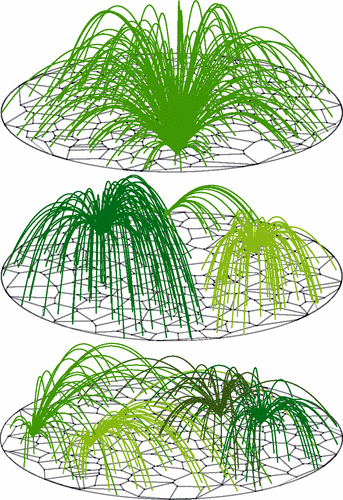
\includegraphics[width = 0.25\linewidth]{图片/polycentric.png}
        \caption{三种城市多中心模式}
    \end{figure}
\end{frame}
\begin{frame}{城市多中心性:场所“供给”市民的一个实例}
    Fujita和Ogawa1982年的模型对多中心问题进行建模\footnote{Modeling the Polycentric Transition of Cities, Rémi Louf and Marc Barthelemy, Phys. Rev. Lett. 111, 198702}:一个人搬到这个城市,会选择住在$i,$ 工作在$j$,使得\[Z_0 = W(j)-C_R(i)-C_T(i,j)\]达到最大。自左到右是:效用,$j$的工资,$i$的租金,$i$到$j$的通勤费用。通勤费用一般来讲正比于欧式距离:$C_T(i,j) = td_{ij}$.

    $i$处定居的人找一个$j$处的工作就会要求$Z_{ij}$达到最大,其中\[Z_{ij} = W(j)-C_T(i,j)\]
\end{frame}

\begin{frame}{城市多中心性:场所“供给”市民的一个实例}
城市中心的个数\footnote{Modeling the Polycentric Transition of Cities, Rémi Louf and Marc Barthelemy
Phys. Rev. Lett. 111, 198702}:

    \begin{align}
        \frac{L}{l}(\frac{P}{(k-1)c})^\mu&>\max_{j\in\{1,2,\ldots,k-1\}}(\eta_j)-\eta_k\notag\\
    (ave({\eta_1-\eta_k})&=\frac{k-1}{N_c+1})\notag\\
    \bar P_k &= P^{*}(k-1)^{\frac{1}{\mu}+1}\notag\\
    k&\sim(\frac{\bar P}{P^{*}})^\frac{\mu}{\mu+1}
    \end{align}
\end{frame}

\begin{frame}{启示}
    用关于“人”的非线性关系探究产业依存关系:不同的超线性关系有着不同的超线性指数
    
    \vspace{0.5cm}
    是否较低的指数的超线性关系是较高指数的超线性关系的“原因”?
\end{frame}

%%%%%%%%%%%%%%%%%%%%%%%%%%%%%%%%%%%%%%%%%%%%
\section{城市的发展:分化与博弈}

\begin{frame}{城市化会进行到底吗?}
    \begin{itemize}
        \item 城市工作的“效益”会随着人员过剩而稀释
        \item 终极状态是三大产业效益相同?
        \item 城乡交通条件改善
        \item ……
    \end{itemize}
\end{frame}

\begin{frame}{城市发展是路径依赖的}
    \begin{itemize}
        \item 城市生态系统与动物界的生态系统的区别:城市的基础设施建设并非产出的规模效应,而是政府满足的大众需要。进而比自然界多一个“层级”
        \item 基础设施建设“完成”时,依然有价值。
        \item 技术发展、产业丰富的过程中,城市空间是相对固定的。
    \end{itemize}
\end{frame}

\begin{frame}{城市发展的多样性、稳定性、过程性}
    城市发展的后续阶段会出现一些问题:
    \begin{itemize}
        \item 城市可以使得群体的智慧组合完成更高价值的产出,但更异质性的人口本身会更稳定吗\footnote{欧洲涌入的大量难民}?
        \item 技术发展、产业丰富的过程中,城市空间是相对固定的。固定的工业园区,在行业形势的变化下也会被废弃。城市空间如何重新组织?
        \item “三个和尚没水喝”?
    \end{itemize}
\end{frame}

\begin{frame}{城市也会演替}
    时序钟\footnote{Batty, M. Rank clocks. Nature 444, 592–596 (2006)}
    \begin{figure}
        \centering
        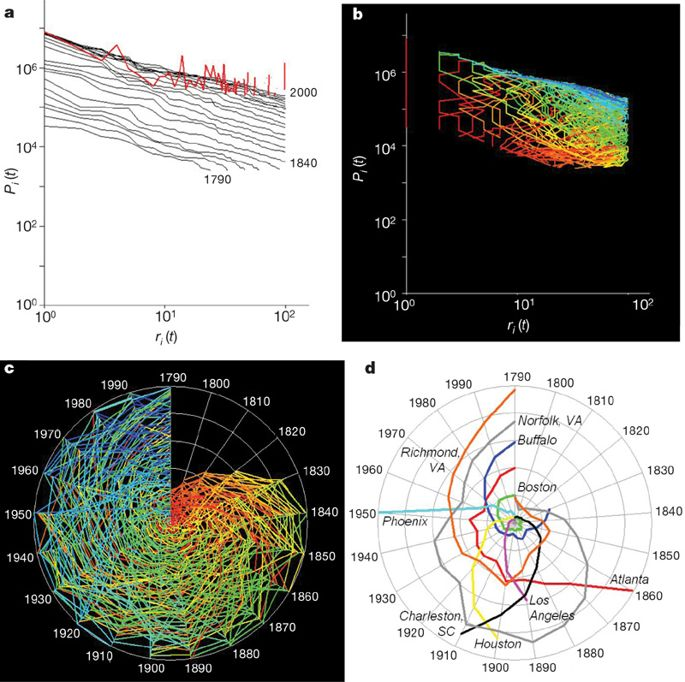
\includegraphics[width = 0.4\linewidth]{图片/rankclocks.jpg}
        \caption{每条线代表一年的城市排名与城市规模的关系。红色线是1950年的城市排名与2000年的人口构成的点对练成的线。(b)是不同城市位序随时间的变化规律。(c)则是序时钟。每个点到圆心的距离代表它的排名。(d)图是几个城市的序时钟轨迹。}
    \end{figure}
\end{frame}

\begin{frame}{生态系统稳定性的模型}
    人工生成的系统\footnote{MAY, R. Will a Large Complex System be Stable?. Nature 238, 413–414 (1972)}:\[\frac{dx}{dt} = Ax\]
    $A$: 均值设置为\(0\),方差的均值设置为\(\alpha\)

    均衡:
    \begin{itemize}
        \item 当且仅当\(A\)的所有特征值都有负的实部,系统是稳定的
        \begin{itemize}
            \item 全局负反馈机制
        \end{itemize}
        \item 有“分块”结构时,稳定性会更高。
        \begin{itemize}
            \item 结构化、(空间)独立,有助于系统稳定
            \item 城市相同产业集中、不同产业相离,有助于城市的“稳定”\footnote{Papadopoulos, F., Kitsak, M., Serrano, M. et al. Popularity versus similarity in growing networks. Nature 489, 537–540 (2012)}
        \end{itemize}
    \end{itemize}
\end{frame}

\begin{frame}{空间演化博弈}
    空间混沌\footnote{Nowak, M., May, R. Evolutionary games and spatial chaos. Nature 359, 826–829 (1992)}
    \begin{figure}
        \centering
        \includegraphics[width = 0.9\linewidth]{图片/spatial_prisoners_dilemma.png}
        \caption{局部交互导致的空间囚徒困境。不好的社会价值观念下,初始人口比例(10\%自私者,90\%合作者)变成大部分都是自私者。万幸,城市的组织(人群交互的复杂性)使得这种“自然法则”很难出现。}
    \end{figure}
\end{frame}

\begin{frame}{永续公地悲剧}
    空间因素在生态中的真正意义还少有人解释。但引入空间因素后,一些社会学上的困境可能有不同的解释\footnote{Spatial Interactions and Oscillatory Tragedies of the Commons, Lin, Yu-Hui and Weitz, Phys. Rev. Lett.122.14.148102,2019}。
    \begin{itemize}
        \item 生态的时间性:系统在演化的过程中存在着周期性。这意味着区域发展过程存在着势能积累。
        \item 空间性给系统提供了缓冲空间,使得势能可以积累。
    \end{itemize}
    自然系统的弹性来源于系统的空间性。
    \begin{figure}
        \centering
        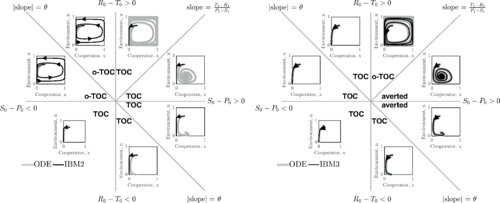
\includegraphics[width = 0.6\linewidth]{图片/toc.png}
        \caption{空间资源和环境的资源的相互关系可以使人类社会走出公地悲剧。}
    \end{figure}
\end{frame}

\begin{frame}{工具}
    \begin{itemize}
        \item 空间分布变迁:演化方程
        \item 产业结构调整:纳什均衡计算
        \item 将未来新形成的产业纳入研究范围:矩阵稀疏化
        \item ……
    \end{itemize}
\end{frame}

\section{总结}

\begin{frame}{总结}
    \begin{itemize}
        \item 城市发展的不同阶段有着不同的性质,需要不同的建模方式
        \begin{itemize}
            \item 初期大空间范围上人口聚集,\textbf{涌现}城市:人口迁移模型、生成模型
            \item \textbf{中期}城市内部复杂机理的形成,城市方式的特有优势(规模效应)使得城市出现城市内出现非线性行为:动力学/因果分析
            \item 逐渐出现基础设施建设放缓(基本完成)的城市体,已有条件下如何改进城市结构:空间演化博弈、生态系统稳定性理论
        \end{itemize}
        \item 人类社会的价值观念集中体现在城市内。如何进行价值建设,使得“公地悲剧”停留在“永续公地悲剧”阶段,应成为我们永恒的主题。
        \item 由于社会价值观念也在随时间演化,城市化也可能放缓,甚至可能停止。我们的研究可能需要根据新的原理重新组织数理工具。
    \end{itemize}
\end{frame}

\begin{frame}
    \begin{center}
    \LARGE{请老师们批评指正!}
    \end{center}
    
\end{frame}

\bibliographystyle{plain}
\bibliography{../references.bib}
\end{document}
